Das Ergebnis der Umsetzung zur Schaffung einer Erweiterung mit Hilfe eines Signatur-Tablets und der Sage Office Line ist auf den unten folgenden Abbildungen zu sehen. Die Erweiterung dient zur Erfassung einer biometrischen Unterschrift. Die Verbindung zwischen dem Signatur-Tablet und dem Computer, auf dem die Sage Office Line läuft, wird mit Hilfe eines USB\footnote{Universal Serial Bus: "'serielles Bussystem zur Verbindung eines Computers mit externen Geräten"' \cite{USB}}- oder COM\footnote{Communication Port: serielle Schnittstelle zur Verbindung eines Computers mit externen Geräten (veraltet) \cite{COM}}-Port realisiert. Die Erfassung von biometrischen Unterschriften ist in dem Standardbereich Verkauf der Sage Office Line und im Zusatzmodul der FZP Vermietung möglich. Auf der Abbildung 12 sieht man den Arbeitsablauf zur Erfassung einer biometrischen Unterschrift im Bereich Verkauf. Die Erfassungsmaske erreicht man über die Schaltfläche Beleg $\rightarrow$ Extras $\rightarrow$ FZP Unterschrift am unteren Rand der Auftragserfassungsmaske. Die Schnittstelle prüft, ob ein Signatur-Tablet verfügbar ist. Nach der Prüfung kann die Unterschrift des Käufers erfasst werden. Anschließend wird die Unterschrift nach der Erfassung auf dem Bildschirm sichtbar. Zum Schluss bestätigt der Kunde die elektronische Unterschrift mit biometrischen Merkmalen. Mit der Bestätigung des Kundens wird die Unterschrift im System gespeichert. Die elektronische Unterschrift wird beim Ausdruck der Verkaufsbelege im Bereich Unterschrift mit ausgegeben. Der Arbeitsablauf zur Erfassung einer digitalen Signatur im Bereich Vermietung verläuft gleichermaßen wie im Bereich Verkauf (siehe Abbildung 13).

\begin{figure}[!ht]
    \centering
    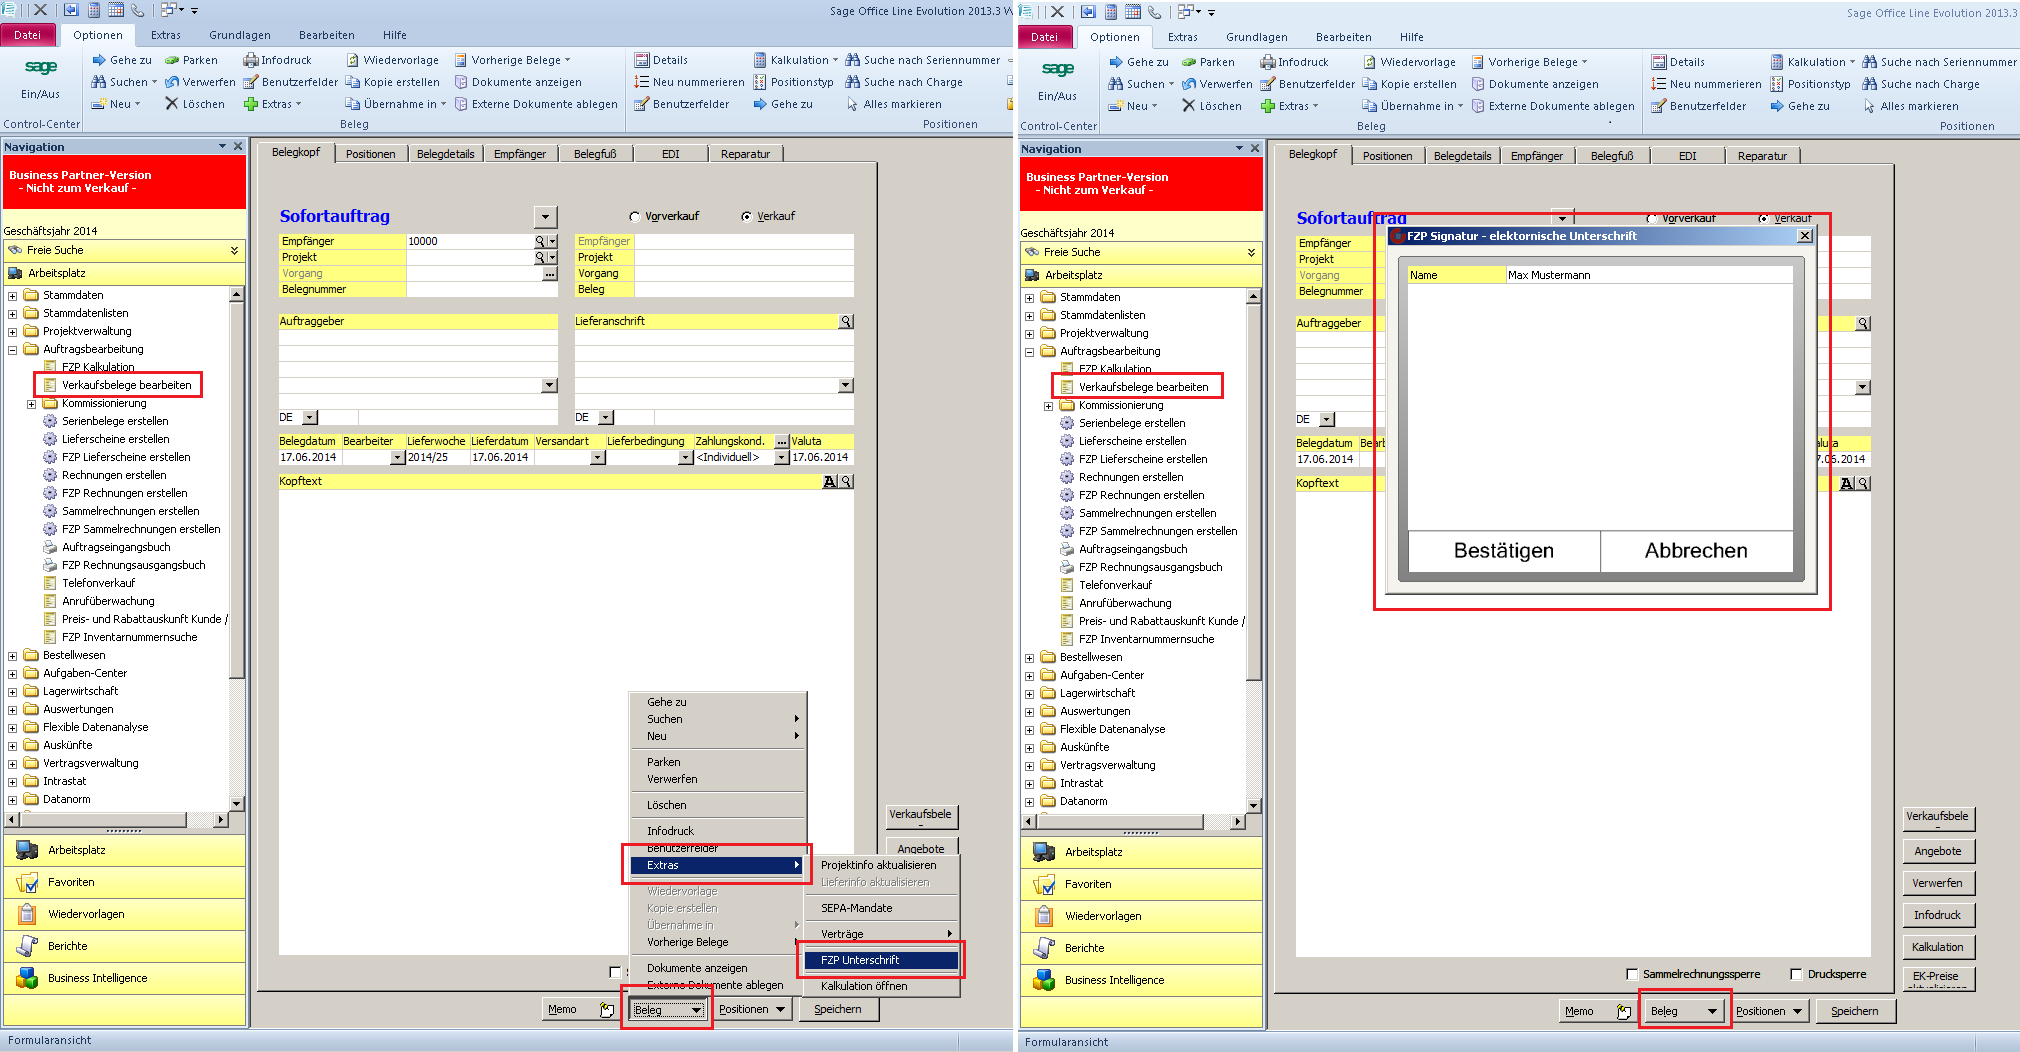
\includegraphics[height=270pt, width=\textwidth]{DigiSigVKBeleg3.png}
    \caption[Ablauf Erfassung digitale Signatur in Sage Office Line (Verkauf)]{\small{Ablauf Erfassung digitale Signatur im Bereich Verkauf in Sage Office Line}}
\end{figure}

\begin{figure}[!ht]
    \centering
    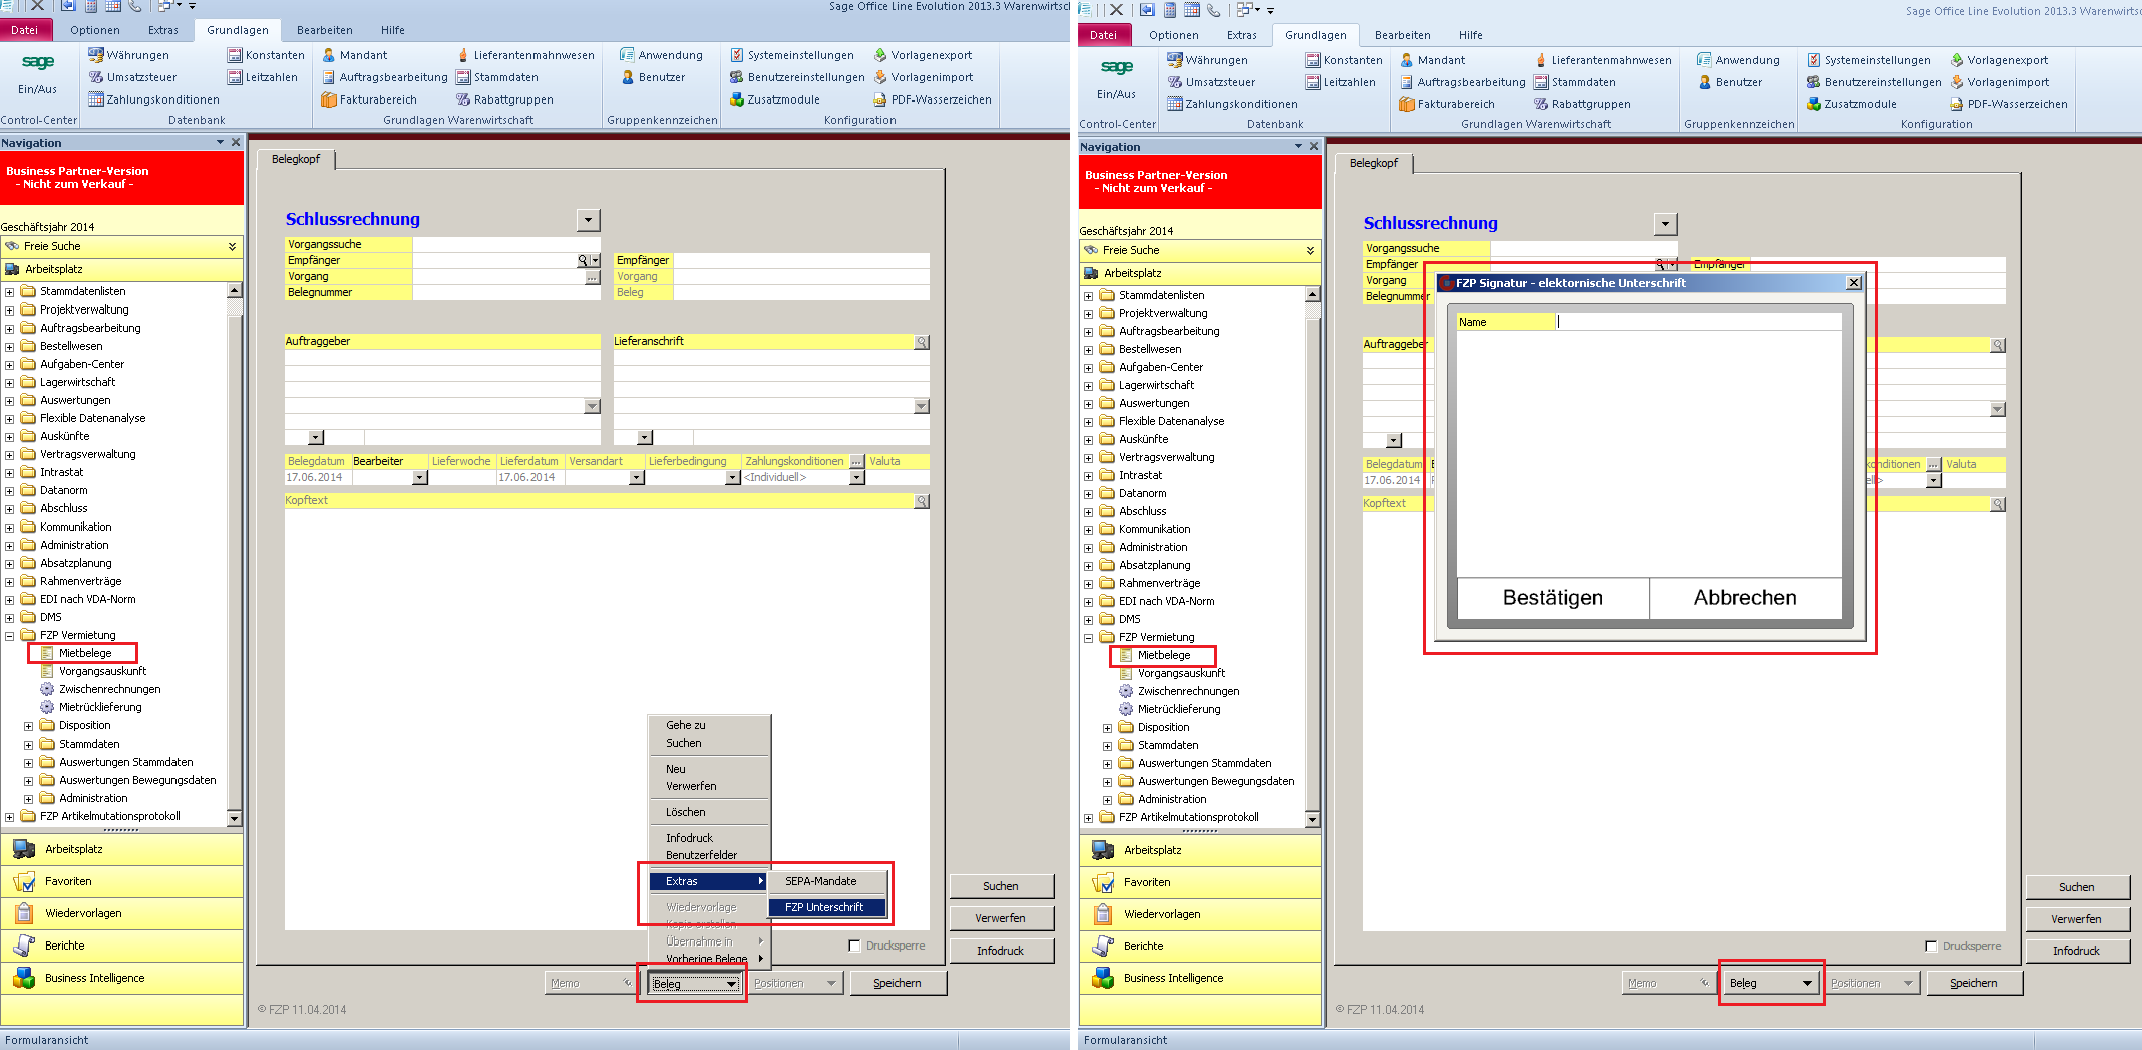
\includegraphics[height=270pt, width=\textwidth]{DigiSigVMBeleg3.png}
    \caption[Ablauf Erfassung digitale Signatur in Sage Office Line (Vermietung)]{\small{Ablauf Erfassung digitale Signatur im Bereich Vermietung in Sage Office Line}}
\end{figure}